{ %section1_2
	\subsection{Terms and Definitions}
	\par\textbf{Parallel computing} -- 
A method of organizing calculations in which the program is a set of interacting modules that work simultaneously. Typically, the concept of concurrency may include:
		\begin{enumerate}

			\item\textbf{Instruction level parallelism} -- one processor core can execute several instructions simultaneously. For example, this technology is implemented in Intel Pentium 4 processors.
			\item\textbf{Hypertreading} -- one processor core is designed so that it can do the work of two threads at once. Implemented in the Intel Core i7 series processors. When performing laboratory work, it is important to disable this in the BIOS (if the processor is compatible with this technology), since it significantly affects the performance of parallel acceleration and efficiency.
			\item\textbf{Multi core programming} --  a method for solving computational problems with simultaneous execution of program parts on different physical computing cores. All cores have shared memory banks, as they are located on the same computer. It includes the case of a multi-core processor architecture and a multi-processor architecture of a system in which there are several processors, since in both cases the program runs on several cores of one or many processors, but on one physical computer.
			\item\textbf{Distributed computing} -- a way to solve time-consuming computing problems using several computers, most often combined into a parallel computing system. Different parts of the program can run on different computers.
		\end{enumerate}
Usually the last two concepts are physically implemented using architectures \textit{SMP} and \textit{MMP}. More details about these architectures can be found in the next section.
	\par It is important to see difference between the concepts of parallel compu-ting and parallel technologies. Let  analyze the following concepts, which, although they are parallel technologies (at the core or internuclear interaction level), however, are not parallel calculations, but often \ textbf {by mistake} are assigned to them:
		\begin{itemize}
			\item\textit{Pipeline data processing (superscalarity)} represents the simultaneous processing by the processor of several instructions, in which at one time for each of the instructions a different execution step is performed. For example, if any processor can simultaneously receive, decode, and execute an instruction, then when it receives the first instruction, it can decode the second and execute the third (Figure~\ref {pipelineExample:image}). This way of organizing calculations is not parallel computing, because the instructions are still executed sequentially, and only one core is involved.
				\begin{figure}[H]
					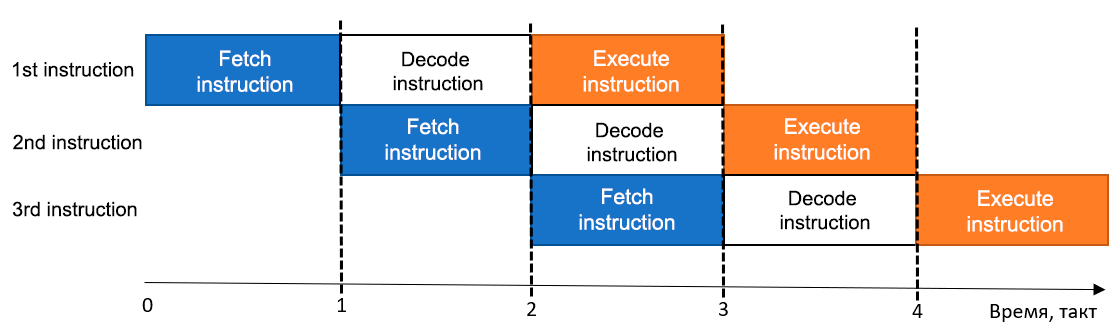
\includegraphics[width=1\linewidth]{pipelineExample}
					\caption{\textit{Instruction pipelining}}
					\label{pipelineExample:image}
				\end{figure}
			\item\textit{SIMD-etensions (MMX, SSE)} provide concurrency at the data level. For example, a processor can simultaneously multiply 4 numbers instead of one using the SSE instruction. However, the command flow still remains single, i.e. one program instruction is executed in a period of time, which is not the case of parallel computing.
			\item\textit{Preemptive Multitasking} organized by the operating system. Several processes are in the execution queue and the OS decides how to manage the processor time between them. If the first thread is given a higher priority than the second, then the OS will allocate more time to execute the first thread, only one thread will be executed at a time, therefore, preemptive multitasking is also not included in the concept of parallel computing.
		\end{itemize}
	\par Various parallelization technologies are used to organize parallel computing:
		\begin{itemize}
			\item\textbf{Process} -- the most heavyweight mechanism used for parallelization. Each process has its own independent address space, so data synchro-nization between processes is long and complicated. May include several threads of execution.
			\item\textbf{Thread.} It runs independently of other threads, but has a common address space with other threads in the same process. At this level, data synchronization mechanisms are used (will be discussed later).
			\item\textbf{Fiber} -- lightweight thread of execution. Like threads, fiber has a common address space, however, it uses joint multitasking instead of preemptive one. The OS does not switch the context from one thread to another, instead, the main thread itself allocates time for the child fiber to work, or is blocked logically (that is, the programmer controls the fiber life cycle). Also, all fibers work on one core, unlike threads, which can work on different kernels.
		\end{itemize}
	\par For a better understanding of threads, we will schematically consider its life cycle. Figure~\ref{threadLifecycle:image} shows that the thread can be in three states - running, waiting and ready. After creating the thread, it is in a ready state. Then, the OS decides to change its state (clarifying multitasking). For fiber, the life cycle is the same, but the programmer or synchronization mechanisms control the transitions between them.
	\par Different standards of programming languages can add new states to the life cycle of threads, for example, blocking a thread, interrupting a thread, and others, but the general scheme of work remains the same.
		\begin{figure}[H]
			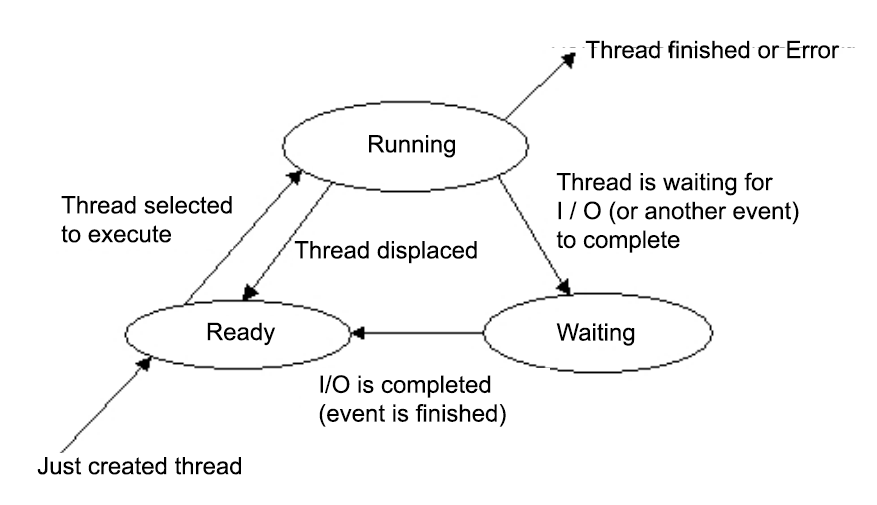
\includegraphics[width=0.9\linewidth]{threadLifecycle}
			\caption{\textit{Thread lifecycle}}
			\label{threadLifecycle:image}
		\end{figure}
	\par Among programmers there are concepts of \textbf{thread-safe} and \textbf{reenterable} functions, however, they may have different meanings in different communities. Table~\ref{threadSafeReentrant:table} provides definitions from different sources.
	\begin{table}[H]
		\caption{Definitions of thread-safe and reenterable functions}
		\label{threadSafeReentrant:table}
		\begin{center}
			\begin{tabularx} {\textwidth} { |c|X|X| }
				\hline 
		\textbf{	Source of definition}	& \textbf{Thread-safe} & \textbf{Reenterable} \\ 
				\hline 
				Qt & Inside the function, all common variables are accessed strictly sequentially, and not in parallel (Thread-safe is reenterable, but not vice versa)  &  Function is called by multiple threads at the same time the correct operation is guaranteed only if the threads do not use shared data \\ 
				\hline 
			Linux	&  The function shows the correct results, even if called by several threads at the same time. & The function shows the correct results, even if re-called internally. \\ 
				\hline
			POSIX	& \center{ ? } & The function shows the correct results, even if called by multiple threads at the same time. \\ 
				\hline 
			\end{tabularx} 

		\end{center}
	\end{table}
	\par Consider examples of functions that fit the definition of the Linux community.
	\begin{figure}[H]
		\lstinputlisting{swapExample1.cpp}
	\end{figure}
	\par This function is not thread safe, not reentrant, because all threads calling it will use the common variable \texttt{t}. If you call the function inside itself, then the value of t is overwritten and the parent function will not work correctly. Let's try to fix these errors by declaring the "\texttt{t}"\ variable of the \texttt{\textunderscore \textunderscore threadint} type.
	\begin{figure}[H]
		\lstinputlisting{swapExample2.cpp}
	\end{figure}
	\par Now the compiler will create a copy of the variable for each thread t and the function will become thread safe, however, it is still not reentrant for the same reason. We will save the value of the global variable t at the beginning of the function and restore it at the end.
	\begin{figure}[H]
		\lstinputlisting{swapExample3.cpp}
	\end{figure}
	\par The new function is reentrant, but again non thread-safe. Finally, we give an example of a standard and proper implementation of \texttt{swap()}, which is thread safe and reentrant:
	\begin{figure}[H]
		\lstinputlisting{swapExample4.cpp}
	\end{figure}
}
